

\documentclass[twoside]{article} %---original command 

% the preamble which specifies packages and parameters for the document
\usepackage{graphics}
\usepackage[pdftex]{color,graphicx}
\usepackage{amsthm}
\usepackage{relsize}
\usepackage{amsmath}
\usepackage{amssymb}
\usepackage{framed}

% for inserting URL's into a page
\usepackage[colorlinks=true, linkcolor=blue, citecolor=blue]{hyperref}

% for numbering lists with (a) (b) (c) and other such nice things
\usepackage[inline]{enumitem}
% optional [inline] option is to get the enumerate* environment (or *enumerate; something like that)

% for blackboard 1's to use with indicator functions
\usepackage{bbold}

%	adds script font, useful e.g. for defining normal RV's or sigma-algebras, \mathscr
\usepackage{mathrsfs}

%----we require the package mathtools in order for the following
%DeclaredPairedDelimiter thing to work, e.g. absolute value and norm
\usepackage{mathtools}
% We also require mathtools for \shortintertext to work

%---required for the commands in the formatting preamble:
\usepackage{fancyhdr}

%-------------Discussion of reasons for using this pacakge can be found here: https://tex.stackexchange.com/questions/29973/more-than-one-optional-argument-for-newcommand or here: https://tex.stackexchange.com/questions/145175/optional-arguments-xparse-vs-xargs  ----------
\usepackage{xargs}
%---------------------Long term, using xparse might be a better implementation
%---use it for the headers and footers commands

%---needed for the custom block quote things. the most argument is as recommended in the answers here:
%--- https://tex.stackexchange.com/a/238296/103825   and  here:  https://tex.stackexchange.com/a/265804/103825
\usepackage[most]{tcolorbox}


% https://tex.stackexchange.com/questions/3238/bm-package-versus-boldsymbol
% This answer says this has to be loaded after all font packages to work correctly: https://tex.stackexchange.com/a/179337
\usepackage{bm}

% https://emacs.stackexchange.com/a/28287/18629
\usepackage{subcaption}

% https://tex.stackexchange.com/questions/192570/cant-force-image-to-be-inserted-here-even-with-using-beginfigureh
\usepackage{float}
%---uses geometry package to set margins and some such
\usepackage[lmargin = 1in, textwidth = 6.5 in, textheight = 8.5 in]{geometry}
% got rid of his setting the top margin to .6in because I think it made the later pages with the fancy headers look ugly

%---in order to get subsections labeled with (a) (b) (c) by default
\renewcommand{\thesubsection}{ (\alph{subsection})}

%---says not to indent paragraphs
\setlength{\parindent}{0 in}

%---set up headers and footers for pages further into the document:

% \headerfooter{ Class/Course }[optional: problem set, assignment, homework]{ number of problem set }{ due date }[your name]
\newcommandx{\headerfooter}[5][2={Problem Set }, 5={William Krinsman} ]{
\pagestyle{fancy}
\lhead{#2 #3}
\rhead{#4}
\chead{}
\lfoot{#5}
\cfoot{#1}
\rfoot{Page \thepage}

}
%---uses the package fancyhdr
%---also uses package xargs for the newcommandx with the optional parameters
%---same command structure as the \HW command


%---uses the package tcolorbox
%---follows exactly answers here: https://tex.stackexchange.com/a/265804/103825 and here: https://tex.stackexchange.com/a/238296/103825 except that environment name is different
\definecolor{block-gray}{gray}{0.85}
\newtcolorbox{blockquote}{colback=block-gray,grow to right by=-10mm,grow to left by=-10mm,
boxrule=0pt,boxsep=0pt,breakable}
%--- see the documentation for explanation of all of the parameter values: https://mirror.hmc.edu/ctan/macros/latex/contrib/tcolorbox/tcolorbox.pdf
%			New math operators

%new, specialized math commands:
%----argmin
\DeclareMathOperator*{\argmin}{\arg\!\min}
%----argmax
\DeclareMathOperator*{\argmax}{\arg\!\max}
%----partial derivatives
\newcommand{\partialderivative}[2][]{\frac{ \partial #1   }{ \partial #2  } }

%----note 1: the following commands require mathtools package
%----note: the DeclarePairedDelimiter and thus the mathtools package are helpful because of this: https://tex.stackexchange.com/questions/2607/spacing-around-left-and-right

%----absolute value
\DeclarePairedDelimiter\absolutevalue{\lvert}{\rvert}
%----norm
\DeclarePairedDelimiter\norm{\lVert}{\rVert}
%----floor
\DeclarePairedDelimiter\floor{\lfloor}{\rfloor}


%			Commonly used symbols

%	real numbers
\newcommand{\reals}{\mathbb{R}}
%	natural numbers
\newcommand{\naturals}{\mathbb{N}}
%	integers
\newcommand{\integers}{\mathbb{Z}}
% 	switches the default epsilon to be the good epsilon and the backup epsilon to be the bad epsilon
\let\otherepsilon\epsilon
\let\realepsilon\varepsilon
\let\varepsilon\otherepsilon
\let\epsilon\realepsilon
% independence sign -- don't quite understand how works, but see here: https://tex.stackexchange.com/questions/79434/double-perpendicular-symbol-for-independence
\newcommand\independent{\protect\mathpalette{\protect\independenT}{\perp}}
\def\independenT#1#2{\mathrel{\rlap{$#1#2$}\mkern6mu{#1#2}}}

% Matrix algebra

% denote rows of a matrix
\newcommand{\row}[1]{(\!\overset{\ \Rightarrow}{#1} \!)}
% denote columns of a matrix
\newcommand{\column}[1]{(\! #1 ^{\Downarrow})}  


% 			Probability Theory

%	expectation operator
\newcommand{\expectation}{\mathbb{E}}
%	probability measure
\newcommand{\probability}{\mathbb{P}}
% indicator functions.  NOTE: this requires package bbold for \mathbb{1} to work
\newcommand{\indicator}[1]{\mathbb{1}_{#1}}
% Variance
\newcommand{\variance}{\operatorname{Var}}
% Covariance
\newcommand{\covariance}{\operatorname{Cov}}
% independent and identically distributed
\newcommand{\iid}{\overset{i.i.d.}{\sim}}
% normal distribution
\newcommand{\gaussian}[2]{\mathscr{N}\left(  #1, #2  \right)}

%			Equation formatting

%	simplified procedure for creating (square bracket shaped) matrices
\newcommand{\Matrix}[1]{  \begin{bmatrix}  #1  \end{bmatrix}  }

%	simplified procedure for putting expressions into parentheses
\newcommand{\parentheses}[1]{  \left(   #1  \right)   }
%	simplified procedure for putting expressions into square brackets
\newcommand{\brackets}[1]{  \left[   #1  \right]   }

% 	load the array package, required for solution given below for equation formatting, see here: https://tex.stackexchange.com/questions/44407/make-every-element-of-an-array-displaystyle
\usepackage{array}
%    also  loading the longtable package for allowing page breaks, see here: https://tex.stackexchange.com/questions/317121/automatically-adding-page-breaks-into-long-array-environments
% did not actually work, it just messed everything up, because interpreter doesn't think longtable is math mode or whatever
% apparently longtable is not designed to be math mode? https://tex.stackexchange.com/questions/155298/math-mode-in-longtabu
% so if I want to use longtable instead of array here, it would require more than just replacing ``array'' with  ``longtable''.


%	waste less time setting up the formatting for equations
\newenvironment{formulae} [1] [3] {
	
	% See array package documentation: http://mirrors.rit.edu/CTAN/macros/latex/required/tools/array.pdf
	% creates three new column types, which are just the regular column types, but with displaystyle inserted automatically before each entry
	\newcolumntype{C}{>{\displaystyle}c}
	\newcolumntype{L}{>{\displaystyle}l}
	\newcolumntype{R}{>{\displaystyle}r}

        % See answer here: https://tex.stackexchange.com/a/267485
       \begingroup\abovedisplayskip=-6pt \abovedisplayshortskip=-6pt \belowdisplayshortskip=-3pt \belowdisplayskip=-3pt
       % https://tex.stackexchange.com/questions/51682/is-it-possible-to-pagebreak-aligned-equations
       %\allowdisplaybreaks
       % above (allowdisplaybreaks) doesn't work though because supposedly only works for the environments from amsmath package unfortunately

	\[  \begin{array}{R*{\numexpr #1 -2}CL<{\smallskip \smallskip}} 
 }{	
 
 % according to here, the size of smallskip (\smallskipamount) is 3.0 pt each, https://tex.stackexchange.com/questions/114569/space-between-paragraphs-local
 % so to delete two unnecessary smallskips after the end of one of these environments arrays, all we have to do is delete 6pt so that is what is now done before ending the array
\\[-6pt]


	\end{array} \]	

\endgroup
 }

% copy-pasted from here: https://tex.stackexchange.com/questions/280819/vertical-space-command-which-is-between-intertext-and-shortintertext
\MHInternalSyntaxOn
\newcommandx{\adjintertext} [3] [1={-15pt}, 2={3pt}]% #1=above skip, #2=below skip, #3=text
{\ifvmode\else\\\@empty\fi
  \noalign{%
    %\penalty\postdisplaypenalty\vskip\belowdisplayskip
    \vskip-\lineskiplimit      % CCS
    \vskip\normallineskiplimit % CCS
    \vskip#1
     \vbox{\normalbaselines
       \ifdim
         \ifdim\@totalleftmargin=\z@
           \linewidth
         \else
           -\maxdimen
         \fi
       =\columnwidth
      \else \parshape\@ne \@totalleftmargin \linewidth
      \fi
      \noindent#3\par}%
    %\penalty\predisplaypenalty\vskip\abovedisplayskip%
    \vskip-\lineskiplimit      % CCS
    \vskip\normallineskiplimit % CCS
    \vskip#2
 }}%
\MHInternalSyntaxOff
% The following macro is used to generate a general header

% \frontbox{ Class/Course }{ type of document }{ number of document type }{ date }[your name][Thing to add before date]
\newcommandx{\frontbox}[6][ 5={William Krinsman}, 6={} ]{
	%----------------- Note how we have to use \newcommandx  (emphasis on the X) instead of \newcommand in order to access the functionality of the xargs package
   \thispagestyle{plain}
   \newpage
   \noindent
%---these three lines I added so that the bottom of the front page matches the bottoms of the other pages 
%  \lfoot{#5}
%   \cfoot{#1}
%  \rfoot{Page \thepage}
%---hopefully makes things look somewhat less ugly
% EDIT: nope, that solution doesn't work -- probably because those commands don't work with pagestyle{plain}, probably only with pagestyle{fancy}
   \begin{center}
   \framebox{
      \vbox{\vspace{2mm}
    \hbox to 6.28in { {  #1
                        \hfill Fall 2018} }
       \vspace{4mm}
       % Add in the specific number of the problem set
       %----------Assignment? Homework? Problem Set?-----------
       \hbox to 6.28in { {\Large \hfill #2 #3  \hfill} }
       \vspace{2mm}
       % Add in the specific due date of the problem set as well as your name
       \hbox to 6.28in { { #5 \hfill #6 #4} }
       % NOTE: changed the above from Due: #4 \hfill #5 because I prefer my name on the left hand side
       % Also got rid of the preceding \it because I thought the italic text was ugly
      \vspace{2mm}}
   }
   \end{center}

}

% The following macro is used to generate headers for the homework and is a specific version of the general header

% \HW{ Class/Course }[optional: problem set, assignment, homework]{ number of problem set }{ due date }[your name]
\newcommandx{\HW}[5][2={Problem Set}, 5={William Krinsman}]{ \frontbox{#1}{#2}{#3}{#4}[#5][Due:] }

% The command structure is as follows:
% \headerfooter{ Class/Course }[optional: problem set, assignment, homework]{ number of problem set }{ due date }[Name]
\headerfooter{}[Final Project]{}{12/06/2018}[Annan Deng, John Canty, Ramasubramanian Balasubramanian, William Krinsman]

% creation of code font following guidelines found here: https://tex.stackexchange.com/a/36031/103825
\newcommand{\code}[1]{\mbox{\texttt{#1}}}

% when the problems you have to answer begin in section 2, uncomment this:
% \setcounter{section}{1}

% don't want this formatting style in the general template for all classes, 
% but do want these assignments to follow her  page format
\renewcommand{\thesubsection}{ \arabic{subsection}.}
\renewcommand{\thesubsubsection}{(\alph{subsubsection})}

\begin{document}

%You can fill in your name in the bracket below and it will print the header HW with your name in it
% In particular the command structure is as follows:
% \HW{ Class/Course }[optional: problem set, assignment, homework]{ number of problem set }{ due date }[Name]
%\HW{PH 240C}[Final Project]{}{12/06/2018}[Ramasubramanian Balasubramanian, John Canty, Annan Deng, William Krinsman]

\title{PH240C Final Project \break\break {\Huge Protein Expression across Disease Groups:} \break \break {\Huge Analysis of the Human Brain Proteome} }
\date{December 6th, 2018}
\author{Ramasubramanian Balasubramanian, John Canty, Annan Deng, William Krinsman}

\maketitle

\section*{Abstract}
\label{sec:abstract}
\addcontentsline{toc}{section}{Abstract}

Patients with neurodegenerative disorders such as Alzheimer’s disease (AD) and Parkinson’s disease (PD) share common physiological and symptomatic similarities, however the molecular pathways linking these diseases are incompletely understood. Recently, a comprehensive quantitative proteomic dataset of the human brain in patients with AD, PD, and AD/PD comorbidity has been publicly released. We will perform exploratory data analysis and modelling in order to identify if there are disease-specific differential protein expression patterns that are associated with AD and PD neuropathologies, reflecting the belief that there may be a relationship between the protein expression patterns between the two diseases. We will then perform Weighted Correlation Network Analysis (WCNA) of the identified protein to assess if there coexpression relationships between subsets of these proteins. Finally, using the PANTHER gene ontology classification system, we will assess whether these proteins exhibit functional relationships. More details of our analysis can be found at our GitHub repository \href{https://github.com/jtcanty/Linear-Modelling-and-Network-Analysis-of-the-Human-Brain-Proteome}{here}. 

\pagebreak

\tableofcontents

\pagebreak

\section{Dataset}
\label{sec:dataset}

The dataset\cite{proteome} that we will be evaluating was obtained by performing Tandem Mass Tag (TMT) isobaric mass spectrometry on brain tissue obtained from individual human donors. Brain tissue samples were obtained from $40$ individual patient samples across two separate brain regions, the Frontal Cortex and the Anterior Cingulate Gyrus). The dataset obtained by using a factorial experimental design, where there are $5$ experimental batches, with two samples of each phenotype (Control Patient, Alzheimer’s Patient, Parkinson’s Patient, Alzheimer’s/Parkinson’s Patient) within each batch. For each batch, a control sample was generated by pooling fractions of all samples in order to generate a global internal standard (GIS) expression measure. Individual data entries are displayed as base-$10$ log-transformed ratios of the obtained peptide counts for the $ij$th sample covariate of interest and the $i$th covariate of the GIS standard. From the Frontal Cortex, $10,100$ unique protein groups were identified, while from the Anterior Cingulate Gyrus, $10,695$ protein groups were identified.


\section{Exploratory analysis and preprocessing}
\label{sec:expl-analys-prepr}

 In the initial portion of this project, we will assess data quality, phenotype and  inter-batch variability by box-plot visualization. We will then assess the raw data and apply quantile normalization samples. Finally, we assess the whether or not disease-trait groups can be discriminated based on gene expression values by applying dimensionality reduction methods. 


\subsection{Data quality and Preprocessing}
\label{subsec:data-qual-vari}

We performed several quality control steps on the data-set before analysis. A large fraction of the gene rows contained batches that consisted of entirely NA or zero values that needed to be removed. We attribute these values to commonly reported issues of label-free mass spectrometry experiments that involve probe bias and reduced coverage of peptides. In order to preserve genes that contained peptide counts for all batches, we removed any gene that had NAs present in any batch. Next, we repeated the process by removing any gene that contained zeros, since these values would result in undefined log-transformed expression measures. In the Frontal Cortex, this process resulted in a final gene count of $6,004$ from an original dataset of $10,100$ genes. In the Anterior Cingulate Gyrus, this resulted in a final gene count of $6230$ genes. 

\subsection{Exploratory analysis}
\label{subsec:exploratory-analysis}

In order to assess our processed data, we visualized the distribution of all fold-change (FC) gene expression values for each patient sample across all disease traits (Ctl, AD, PD, and ADPD) \textbf{ (Fig.1A)}. Upon inspection of the plots, we noticed that all samples had FC gene expression values that were centered around zero, indicating that the experimental effects between batches were significantly reduced by normalizing against a GIS for each batch. However, for a fraction of patient samples, we still observed significant FC gene expression outliers. 

Next, we performed Principle Component Analysis (PCA) on the samples in both the Frontal Cortex and the Anterior Cingulate Gyrus \textbf{(Fig.2A and B)}. A PCA plot of all disease traits did not indicate any clear separation of classes in both tissues. In order to simplify visualization, we then generated pairwise PCA plots between the Control samples and disease-state samples in both tissues \textbf{ (Fig.2C and D)}. In both tissue samples, we observed that clear separation of the Control and AD samples. Similarly, we observed separation of the Control and comorbid ADPD samples. However, when when we analyzed the Control and PD samples, we did not observe clear separation between the two traits.

We then quantitatively assessed the separation between the Control and disease-state samples by applying a Support Vector Machine (SVM) classifier to the PCA plots \textbf{(Fig.2 E and F)}. Consistent with our observations from the PCA plots, we observed that the SVM was able to accurately classify Control samples versus AD and comorbid PDAD samples. However, SVM classifier performed substantially worse with PD samples. Based on these observations, we concluded that the PD samples do not exhibit noticeable variances in gene expression compared to Control samples.

\section{Linear modelling to identify differential expression}
\label{sec:line-modell-ident}

In order to identify differentially expressed genes between Control samples and disease-state samples, we utilized linear models. We  samples as covariates (with parameter coefficientsfor the control, AD, PD, and AD/PD samples) in order to determine the strength of association between each gene and the disease phenotypes. We used two separate linear modelling approaches. First, we modelled each trait as additive categorical random variables: 
\begin{align*}
E[Y^{i}|X^{i}] &= \beta_{Ctl} + \beta_{AD}x_{AD}^{i} + \beta_{PD}x_{PD}^{i} + \beta_{ADPD}x_{ADPD}^{i} \\  
\end{align*}
Where the $x^{i}s$ are indicator variables for the presence or absence of each disease-trait in a sample.Using this approach, we performed linear modelling on each gene, and obtained sample estimators $\hat{\beta}_{Ctl}, \hat{\beta}_{AD}, \hat{\beta}_{PD}, and \hat{\beta}_{ADPD}$. 

We also considered that the changes in gene expression values in the ADPD case may not simply reflect additive changes in from both AD and PD in a linear model. To model this, we considered the comorbid case as an interaction effect between both the AD and PD traits:
\begin{align*}
E[Y^{i}|X^{i}] &= \beta_{Ctl} + \beta_{AD}x_{AD}^{i} + \beta_{PD}x_{PD}^{i} + \beta_{ADPD}x_{AD}^{i}x_{PD}^{i} \\  
\end{align*}
Repeating the same analysis as in the additive case, we obtained sample estimators for the AD, PD, and ADPD cases.

\subsection{Volcano plots to identify differential expression}
\label{subsec:volc-plots-ident}

After obtaining sample estimators  $\hat{\beta}_{Ctl}, \hat{\beta}_{AD}, \hat{\beta}_{PD},$ and $\hat{\beta}_{ADPD}$ for each gene in the in Frontal Cortex and Anterior Cingulate Cyrus, we then computed the the log-fold change and p-value of the fold-change. We performed this calculation for each gene with the disease-state sample estimators against the Control sample estimator:
\begin{align*}
& log_{2}FC( \hat{\beta}_{Ctl},\hat{\beta}_{AD})		&Pval (\hat{ \beta}_{Ctl},\hat{\beta}_{AD}) \\  
& log_{2}FC(\hat{ \beta}_{Ctl},\hat{\beta}_{PD})		& Pval(\hat{ \beta}_{Ctl},\hat{\beta}_{PD}) \\  
& log_{2}FC( \hat{\beta}_{Ctl},\hat{\beta}_{ADPD})   		& Pval(\hat{ \beta}_{Ctl},\hat{\beta}_{ADPD}) \\  
\end{align*}

Next, we plotted our results using volcano plots. We defined a differential expressed gene as any gene expression value where the p-value was less than $\frac{0.05}{nGenes}$ and the $log_{2}$ fold-change was larger than $0.25$ \textbf{(Fig 3.A and B)}.

\section{Weighted correlation network analysis}
\label{sec:weight-corr-netw}

 Using the candidate differentially expressed genes for the PD, AD, and PD/AD disease phenotypes, we will apply weighted correlation network analysis in order to determine if the candidate genes exhibit interesting coexpression patterns. First, using the available WGNA R-package\cite{Langfelder2008}, we will determine whether there are interesting coexpression clusterings between differentially expressed genes for each phenotype. Next, we will assess the clustering size/structure and compare these properties between phenotypes.

\subsection{Analysis of coexpression clusterings}
\label{subsec:analys-coexpr-clust}

\subsubsection{Size and structure of clusterings}
\label{subsec:size-struct-clust}

\subsubsection{Comparison of clusters between phenotypes}
\label{subsec:comp-clust-betw}


\section{Biological functions of differentially expressed genes}
\label{sec:biol-funct-diff}

Using the PANTHER gene ontology database, we identify the functional classifications of the differential expressed genes. We will perform this analysis between all phenotypes in order to comment on genes that may have unique biological roles related to PD, AD, and PD/AD disease states.


\subsection{PANTHER gene ontology database}
\label{subsec:panth-gene-ontol}

The PANTHER project, which we used to identify the biological functions of the differentially expressed genes, has the following purpose\cite{PANTHER}:\\

\begin{blockquote}
  The PANTHER (protein annotation through evolutionary relationship) classification system (\url{http://www.pantherdb.org/}{http://www.pantherdb.org/}) is a comprehensive system that combines gene function, ontology, pathways and statistical analysis tools that enable biologists to analyze large-scale, genome-wide data from sequencing, proteomics or gene expression experiments. The system is built with 82 complete genomes organized into gene families and subfamilies, and their evolutionary relationships are captured in phylogenetic trees, multiple sequence alignments and statistical models (hidden Markov models or HMMs). Genes are classified according to their function in several different ways: families and subfamilies are annotated with ontology terms (Gene Ontology (GO) and PANTHER protein class), and sequences are assigned to PANTHER pathways.
\end{blockquote}

\subsection{Functional classifications of differentially expressed proteins in frontal cortex}
\label{subsec:funct-class-diff}

\subsubsection{Alzheimer's disease versus controls (Additive and interaction model)}
\label{sec:prot-ident-alzh}

\paragraph{Proteins identified as differentially expressed by both additive and interaction model}

{
\small

\begin{itemize}
\item \href{http://www.pantherdb.org/genes/gene.do?acc=HUMAN\%7CHGNC\%3D6893\%7CUniProtKB\%3DP10636}{P10636}: Microtubule-associated protein tau, associated with microtubule binding and neuron projection.
\item \href{http://www.pantherdb.org/genes/gene.do?acc=HUMAN\%7CHGNC\%3D17056\%7CUniProtKB\%3DQ9Y2J0}{Q9Y2J0}: Rabphilin-3A, function undescribed for humans in PANTHER.
\item \href{http://www.pantherdb.org/genes/gene.do?acc=HUMAN\%7CHGNC\%3D2318\%7CUniProtKB\%3DQ9HCH3}{Q9HCH3}: Copine-5, function undescribed for humans in PANTHER.
\item \href{http://www.pantherdb.org/genes/gene.do?acc=HUMAN\%7CHGNC\%3D20318\%7CUniProtKB\%3DQ9H4F8}{Q9H4F8}: SPARC-related modular calcium-binding protein 1, associated with the binding of calcium ions.
\item \href{http://www.pantherdb.org/genes/gene.do?acc=HUMAN\%7CHGNC\%3D4638\%7CUniProtKB\%3DP09211}{P09211}: Glutathione S-transferase P, function undescribed for humans in PANTHER.
\item \href{http://www.pantherdb.org/genes/gene.do?acc=HUMAN\%7CHGNC\%3D9099\%7CUniProtKB\%3DQ9UIW2}{Q9UIW2}: Also known as \href{https://www.uniprot.org/uniprot/Q9UIW2}{PLXNA1 (Plexin-A1)}, associated with axon guidance mediated by semaphorins, nervous system development, signal transducer activity, receptor activity, GTPase activity, pyrophosphatase activity, and many others.
\item \href{http://www.pantherdb.org/genes/gene.do?acc=HUMAN\%7CHGNC\%3D29393\%7CUniProtKB\%3DQ96Q06}{Q96Q06}: Perilipin-4, function undescribed for humans in PANTHER.
\item \href{http://www.pantherdb.org/genes/gene.do?acc=HUMAN\%7CHGNC\%3D11444\%7CUniProtKB\%3DP61764}{P61764}: Syntaxin-binding protein 1, also known as \href{https://www.uniprot.org/uniprot/P61764}{STXBP1}, associated with synaptic vesicle exocytosis and trafficking (as part of synaptic transmission).
\item \href{http://www.pantherdb.org/genes/gene.do?acc=HUMAN\%7CHGNC\%3D2451\%7CUniProtKB\%3DP48729}{P48729}: Also known as \href{https://www.uniprot.org/uniprot/P48729}{CSNK1A1 (Casein kinase I isoform alpha))}, associated with protein kinase activity. Well known to be associated with Parkinson's disease.
\item \href{http://www.pantherdb.org/genes/gene.do?acc=HUMAN\%7CHGNC\%3D16753\%7CUniProtKB\%3DP30041}{P30041}: Peroxiredoxin-6, an enzyme which catalyzes the oxidation via hydrogen peroxide.
\item \href{http://www.pantherdb.org/genes/gene.do?acc=HUMAN\%7CHGNC\%3D2033\%7CUniProtKB\%3DP78369}{P78369}: Claudin-10,  a tight junction protein known to be found in the plasma membrane.
\item \href{http://www.pantherdb.org/genes/gene.do?acc=HUMAN\%7CHGNC\%3D8923\%7CUniProtKB\%3DO43175}{O43175}: D-3-phosphoglycerate dehydrogenase, associated with the synthesis of serine and glycine.
\item \href{http://www.pantherdb.org/genes/gene.do?acc=HUMAN\%7CHGNC\%3D19129\%7CUniProtKB\%3DQ9Y617}{Q9Y617}: Phosphoserine aminotransferase, also associated with the synthesis of serine and glycine, as well as pyridoxal-5 phosphate synthesis and vitamin B6 metabolism.
\item \href{http://www.pantherdb.org/genes/gene.do?acc=HUMAN\%7CHGNC\%3D2482\%7CUniProtKB\%3DP04080}{P04080}: Cystatin-B, known to be a cysteine protease inhibitor.
\item \href{http://www.pantherdb.org/genes/gene.do?acc=HUMAN\%7CHGNC\%3D4288\%7CUniProtKB\%3DO95452}{O95452}: Gap junction beta-6 protein, associated with gap junction channel activity in the plasma membrane.
\item \href{http://www.pantherdb.org/genes/gene.do?acc=HUMAN\%7CHGNC\%3D10661\%7CUniProtKB\%3DP31431}{P31431}: Syndecan-4, a cytoskeletal protein involved in cell adhesion and the extracellular matrix, as well as membrane-bound signalling.
\item \href{http://www.pantherdb.org/genes/gene.do?acc=HUMAN\%7CHGNC\%3D11280\%7CUniProtKB\%3DQ13501}{Q13501}: Sequestosome-1, known to be associated with protein binding in vacuoles in the cytoplasm.
\item \href{http://www.pantherdb.org/genes/gene.do?acc=HUMAN\%7CHGNC\%3D5246\%7CUniProtKB\%3DP04792}{P04792}: Heat shock protein beta-1, involved in multiple signalling pathways as well as sensory and in particular visual perception.
\item \href{http://www.pantherdb.org/genes/gene.do?acc=HUMAN\%7CHGNC\%3D18304\%7CUniProtKB\%3DQ14019}{Q14019}: Coactosin-like protein, involved in the intracellular actin cytoskeleton, in particular with the binding of actin as well as a cytoskeletal component itself.
\item \href{http://www.pantherdb.org/genes/gene.do?acc=HUMAN\%7CHGNC\%3D19663\%7CUniProtKB\%3DQ9UBI6}{Q9UBI6}: Guanine nucleotide-binding protein G(I)/G(S)/G(O) subunit gamma-12, involved in GTPase activity, protein binding, and numerous signalling pathways.
\item \href{http://www.pantherdb.org/genes/gene.do?acc=HUMAN\%7CHGNC\%3D20983\%7CUniProtKB\%3DQ8N987}{Q8N987}: N-terminal EF-hand calcium-binding protein 1, known to be found in the cytoplasm and involved in the regulation of cellular metabolism, given the naming presumably via the binding of calcium. Otherwise little else appears to be described in PANTHER.
\end{itemize}

}

\paragraph{Identified by interaction model but not additive model}

{
\small

\begin{itemize}
\item \href{http://www.pantherdb.org/genes/gene.do?acc=HUMAN\%7CHGNC\%3D17972\%7CUniProtKB\%3DQ9NPD7}{A0A087WWT2}: Neuritin, also known as \href{https://www.uniprot.org/uniprot/A0A087WWT2}{NRN1}, function undescribed for humans in PANTHER.
\item \href{http://www.pantherdb.org/genes/gene.do?acc=HUMAN\%7CHGNC\%3D29167\%7CUniProtKB\%3DQ9Y2K5}{B5MCG9}: R3H domain-containing protein 2, also known as \href{https://www.uniprot.org/uniprot/B5MCG9}{R3HDM2}, function unknown in humans.
\item \href{http://www.pantherdb.org/genes/gene.do?acc=HUMAN\%7CHGNC\%3D29180\%7CUniProtKB\%3DQ9UPV7}{Q9UPV7}: Unnamed, also known as \href{https://www.uniprot.org/uniprot/Q9UPV7}{PHF24 (PHD Finger Protein 24))}, function undescribed for humans in PANTHER.
\end{itemize}

}

\paragraph{Identified by interaction model but not additive model}

None.\\

\begin{figure}[H]
\label{adfigure}
\begin{subfigure}[b]{0.5\linewidth}
\centering
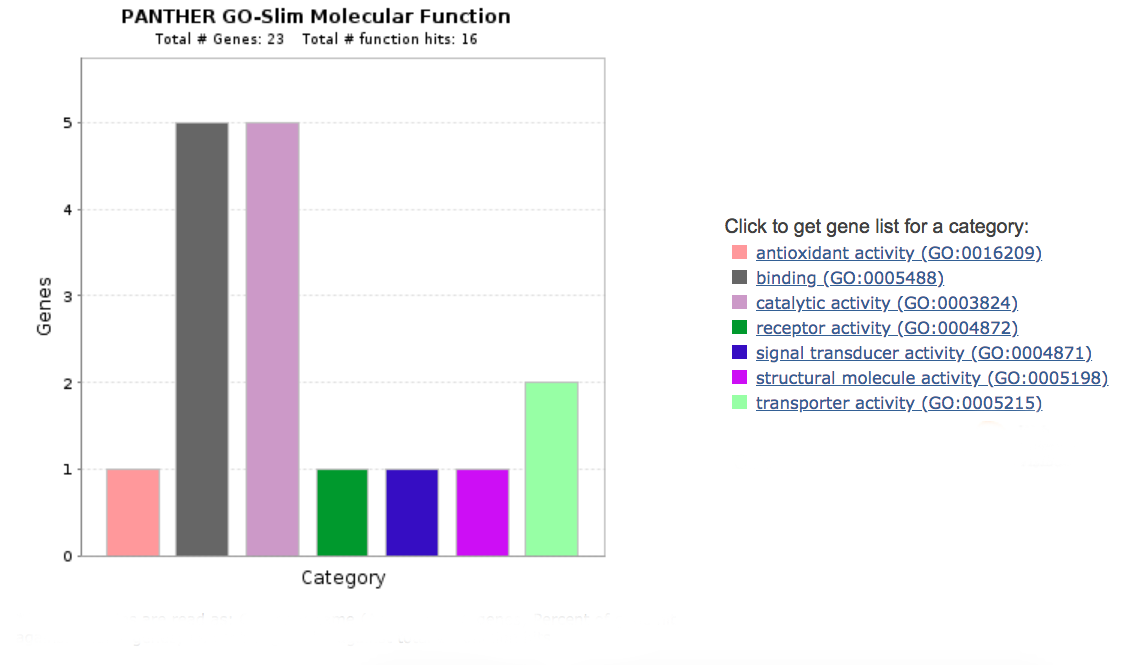
\includegraphics[width=0.9\textwidth]{./Figures/GO/ad/ad1}\par
\end{subfigure}
\begin{subfigure}[b]{0.5\linewidth}
\centering
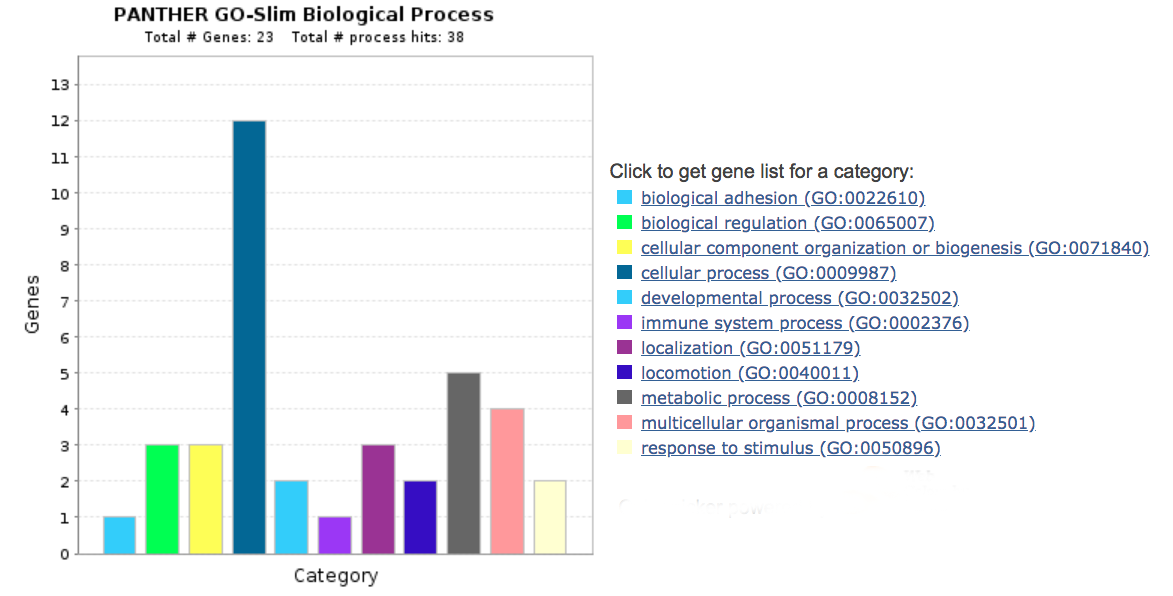
\includegraphics[width=0.9\textwidth]{./Figures/GO/ad/ad2}\par
\end{subfigure}\\
\begin{subfigure}[b]{0.5\linewidth}
\centering
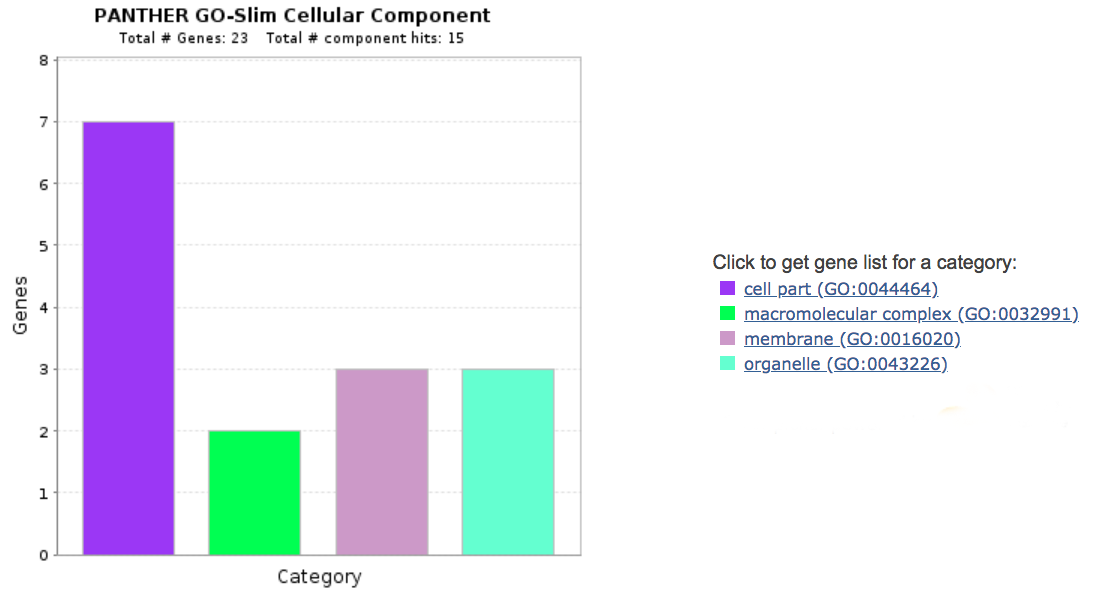
\includegraphics[width=0.9\textwidth]{./Figures/GO/ad/ad3}\par
\end{subfigure}
\begin{subfigure}[b]{0.5\linewidth}
\centering
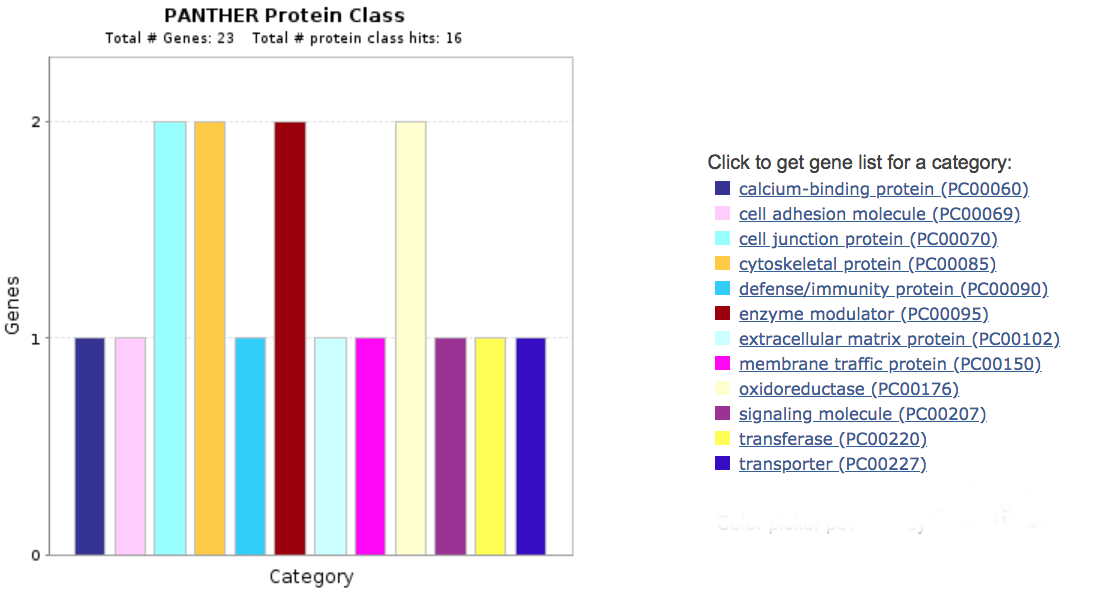
\includegraphics[width=0.9\textwidth]{./Figures/GO/ad/ad4}\par
\end{subfigure}%
\begin{caption}
  {Gene ontologies for proteins found in \ref{sec:prot-ident-alzh}.}
\end{caption}
\end{figure}

\textbf{Comments:} First, it is a good validation of our methodology that it detected the differential expression of the tau proteins, given the extensive prior literature relating these proteins to Alzheimer's disease. It is also noteworthy that protein already well-known to be associated with Parkinson's disease, namely Casein kinase I isoform alpha, was found to be differentially expressed in the frontal cortex of Alzheimer's disease patients who did not also have Parkinson's. This is for two reasons: first, Parkinson's does not seem to affect the frontal cortex, so it is interesting that it might be involved with Alzheimer's in that region of the brain, and second, it provides support for the authors' conjecture that there may be structural similarity/relationship between the development of Alzheimer's and Parkinson's diseases.\\

As for some possible common themes that seem worth mentioning with regards to the biological functions of the differentially expressed proteins, these include calcium-binding, GTPase activity, synthesis of serine and glycine, signalling pathways, protein binding, cellular membrane functions, and the internal and external cytoskeletons.\\

Also, there were several proteins identified as differentially expressed whose function is still relatively unknown, including (but not necessarily limited to) Rabphilin-3A, Copine-5, Glutathione S-transferase P, and Perilipin-4. Our analysis strongly suggests that future research clarifying the biological function of these specific proteins could be relevant to understanding the pathology behind Alzheimer's disease.\\

We see an extremely large overlap between proteins already identified via the additive model as differentially expressed in either Alzheimer's patients or patients with comorbid Alzheimer's and Parkinson's, with the only exception being R3H domain-containing protein 2. Thus this seems to lend further support to the importance of these genes, if only to the extent that their being identified as differentially expressed does not appear contingent upon the exact assumptions of the linear model being used.\\


\subsubsection{Parkinson's Disease versus Controls (Additive and Interaction Model)}

No genes were differentially expressed. This is also a validation of our methodology, since it corresponds to previous work which suggests that there is no manifestation of Parkinson's in the frontal cortex.

\subsubsection{Comorbid Alzheimer's and Parkinson's Diseases versus Controls (Additive and Interaction Model)}
\label{adpd}

{
\small

\begin{itemize}
\item \href{http://www.pantherdb.org/genes/gene.do?acc=HUMAN\%7CHGNC\%3D12684\%7CUniProtKB\%3DO15240}{O15240}: Neurosecretory protein VGF, function undescribed for humans in PANTHER.
\item \href{http://www.pantherdb.org/genes/gene.do?acc=HUMAN\%7CHGNC\%3D20318\%7CUniProtKB\%3DQ9H4F8}{Q9H4F8}: SPARC-related modular calcium-binding protein 1, associated with the binding of calcium ions.
\item \href{http://www.pantherdb.org/genes/gene.do?acc=HUMAN\%7CHGNC\%3D9243\%7CUniProtKB\%3DO14829}{O14829}: Serine/threonine-protein phosphatase with EF-hands 1, associated with apoptosis and intracellular signalling.
\item \href{http://www.pantherdb.org/genes/gene.do?acc=HUMAN\%7CHGNC\%3D17972\%7CUniProtKB\%3DQ9NPD7}{A0A087WWT2}: Neuritin, also known as \href{https://www.uniprot.org/uniprot/A0A087WWT2}{NRN1}, function undescribed for humans in PANTHER.
\item \href{http://www.pantherdb.org/genes/gene.do?acc=HUMAN\%7CHGNC\%3D9476\%7CUniProtKB\%3DQ92743}{Q92743}: Serine protease HTRA1, associated with serine-type proteolysis (peptide and protein breakdown).
\item \href{http://www.pantherdb.org/genes/gene.do?acc=HUMAN\%7CHGNC\%3D5246\%7CUniProtKB\%3DP04792}{P04792}: Heat shock protein beta-1, involved in multiple signalling pathways as well as sensory and in particular visual perception.
\item \href{http://www.pantherdb.org/genes/gene.do?acc=HUMAN\%7CHGNC\%3D11280\%7CUniProtKB\%3DQ13501}{Q13501}: Sequestosome-1, known to be associated with protein binding in vacuoles in the cytoplasm.
\item \href{http://www.pantherdb.org/genes/gene.do?acc=HUMAN\%7CHGNC\%3D29393\%7CUniProtKB\%3DQ96Q06}{Q96Q06}: Perilipin-4, function undescribed for humans in PANTHER.
\item \href{http://www.pantherdb.org/genes/gene.do?acc=HUMAN\%7CHGNC\%3D17056\%7CUniProtKB\%3DQ9Y2J0}{Q9Y2J0}: Rabphilin-3A, function undescribed for humans in PANTHER.
\item \href{http://www.pantherdb.org/genes/gene.do?acc=HUMAN\%7CHGNC\%3D13564\%7CUniProtKB\%3DQ92563}{Q92563}: Testican-2, associated with calcium ion binding, and the inhibition of proteolysis.
\item \href{http://www.pantherdb.org/genes/gene.do?acc=HUMAN\%7CHGNC\%3D2033\%7CUniProtKB\%3DP78369}{P78369}: Claudin-10,  a tight junction protein known to be found in the plasma membrane.
\item \href{http://www.pantherdb.org/genes/gene.do?acc=HUMAN\%7CHGNC\%3D964\%7CUniProtKB\%3DO75936}{O75936}: Gamma-butyrobetaine dioxygenase, known to be associated with the synthesis of certain vitamins.
\item \href{http://www.pantherdb.org/genes/gene.do?acc=HUMAN\%7CHGNC\%3D17187\%7CUniProtKB\%3DQ99784}{Q99784}: Noelin, a phosphate ion receptor and transporter.
\item \href{http://www.pantherdb.org/genes/gene.do?acc=HUMAN\%7CHGNC\%3D13345\%7CUniProtKB\%3DQ14693}{Q14693}: Phosphatidate phosphatase LPIN1, known to be associated with the regulation of transcription.
\item \href{http://www.pantherdb.org/genes/gene.do?acc=HUMAN\%7CHGNC\%3D3978\%7CUniProtKB\%3DO75891}{O75891}: Cytosolic 10-formyltetrahydrofolate dehydrogenase, a catalyst for the transfer of electrons from one molecule to another (oxidation-reduction reactions).
\item \href{http://www.pantherdb.org/genes/gene.do?acc=HUMAN\%7CHGNC\%3D166\%7CUniProtKB\%3DO43707}{K7EJH8}: Alpha-actinin-4, also known as \href{https://www.uniprot.org/uniprot/K7EJH8}{ACTN4}, associated with the morphogenesis of the extracellular matrix/cytoskeleton.
\item \href{http://www.pantherdb.org/genes/gene.do?acc=HUMAN\%7CHGNC\%3D1470\%7CUniProtKB\%3DQ96RR4}{Q96RR4}: Calcium/calmodulin-dependent protein kinase 2, associated with calcium-mediated synaptic transmission.
\item \href{http://www.pantherdb.org/genes/gene.do?acc=HUMAN\%7CHGNC\%3D29180\%7CUniProtKB\%3DQ9UPV7}{Q9UPV7}: Unnamed, also known as \href{https://www.uniprot.org/uniprot/Q9UPV7}{PHF24 (PHD Finger Protein 24)}, function undescribed for humans in PANTHER.
\item \href{http://www.pantherdb.org/genes/gene.do?acc=HUMAN\%7CHGNC\%3D1063\%7CUniProtKB\%3DP30043}{P30043}: Flavin reductase (NADPH), another oxidation-reduction catalyst.
\item \href{http://www.pantherdb.org/genes/gene.do?acc=HUMAN\%7CHGNC\%3D8576\%7CUniProtKB\%3DQ15102}{Q15102}: Platelet-activating factor acetylhydrolase IB subunit gamma, specific function undescribed for humans in PANTHER.
\item \href{http://www.pantherdb.org/genes/gene.do?acc=HUMAN\%7CHGNC\%3D20039\%7CUniProtKB\%3DP40123}{P40123}: Adenylyl cyclase-associated protein 2, known to be involved in the organization and regulation of the intracellular actin cytoskeleton in the cytoplasm.
\item \href{http://www.pantherdb.org/genes/gene.do?acc=HUMAN\%7CHGNC\%3D16280\%7CUniProtKB\%3DQ9NQ86}{Q9NQ86}: E3 ubiquitin-protein ligase TRIM36, specific function undescribed for humans in PANTHER.
\item \href{http://www.pantherdb.org/genes/gene.do?acc=HUMAN\%7CHGNC\%3D9064\%7CUniProtKB\%3DQ9UPR0}{Q9UPR0}:  Inactive phospholipase C-like protein 2, associated with GTPase regulation and several intracellular signalling pathways.
\end{itemize}

}

Even though some of the results are given via gene ID instead of protein ID or vice versa, ultimately the results here are literally identically the same as those for the additive model. This suggests that the two models also should have given identical output for the Alzheimer's only group as well (they gave identical output for the Parkinson's only group too), which strongly suggests that we may have made an error in our analysis (which unfortunately due to time constraints cannot be addressed).\\

Some common themes include regulation and development of the actin cytoskeleton, oxidation-reduction reaction catalysts, and several of the categories mentioned above (e.g. calcium ion binding, GTPase regulators, signalling pathways, vitamin synthesis, protein binding, etc.).\\

The occurrence of several proteins in both this group as well as those differentially expressed with Alzheimer's (e.g. heat-shock protein beta-1, Sequestosome-1, SPARC-related modular calcium-binding protein 1) only could be seen to validate our methodology, since we would expect these two groups to have similar protein expression profiles. Similarly, the occurrence of the unknown function proteins Perilipin-4 and Rabphilin-3A as differentially expressed in both of these groups strongly argues in favor of follow-up studies investigating the function and structure of these proteins.\\

\begin{figure}[H]
\label{adpdfigure}
\begin{subfigure}[b]{0.5\linewidth}
\centering
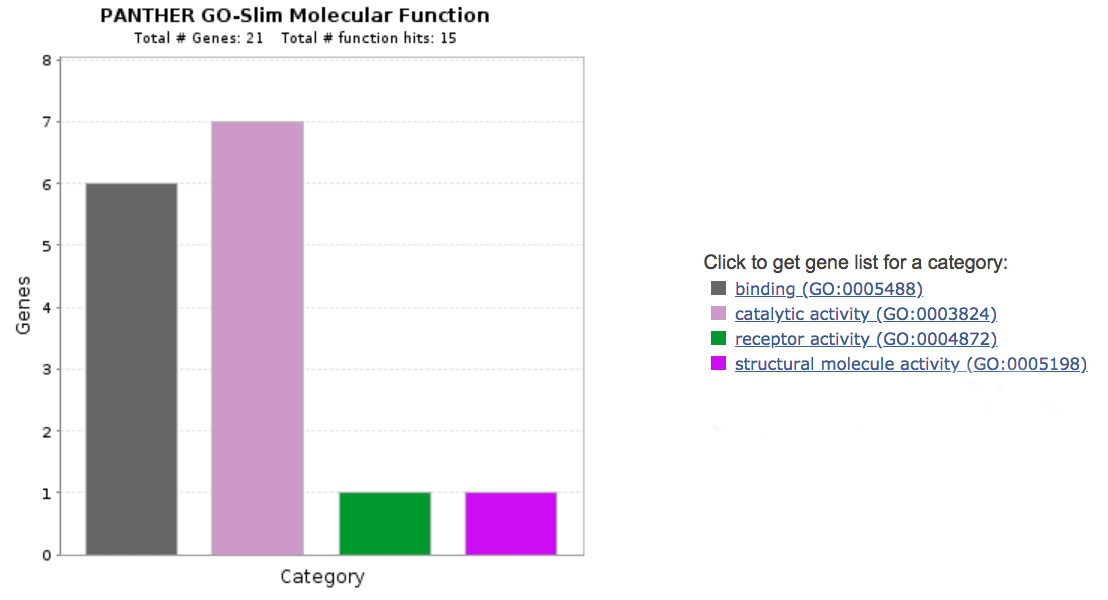
\includegraphics[width=0.9\textwidth]{./Figures/GO/adpd/adpd1}\par
\end{subfigure}
\begin{subfigure}[b]{0.5\linewidth}
\centering
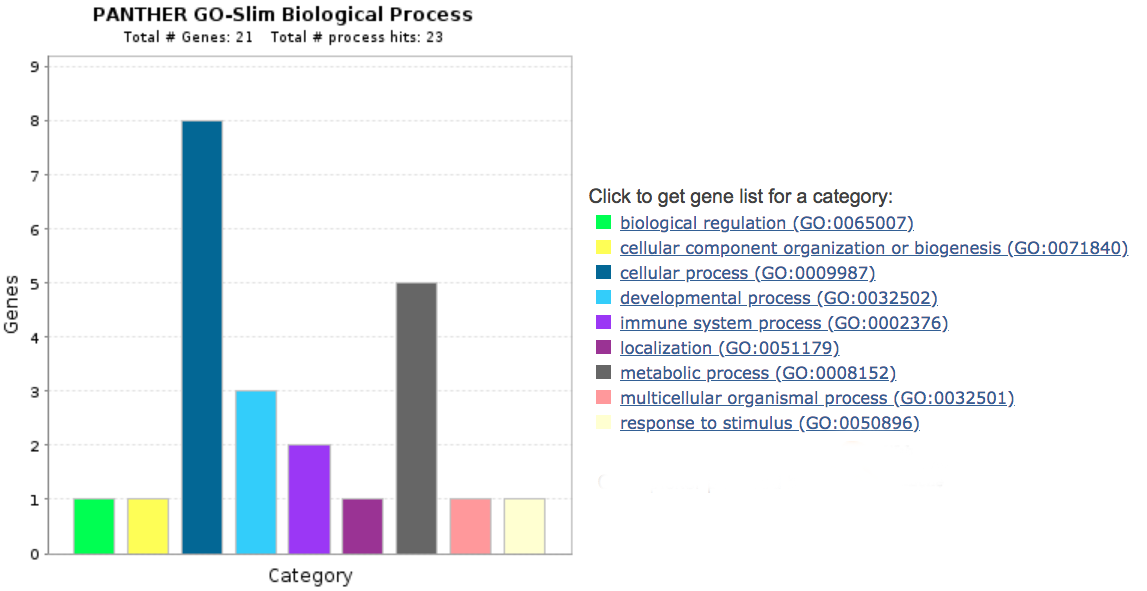
\includegraphics[width=0.9\textwidth]{./Figures/GO/adpd/adpd2}\par
\end{subfigure}\\
\begin{subfigure}[b]{0.5\linewidth}
\centering
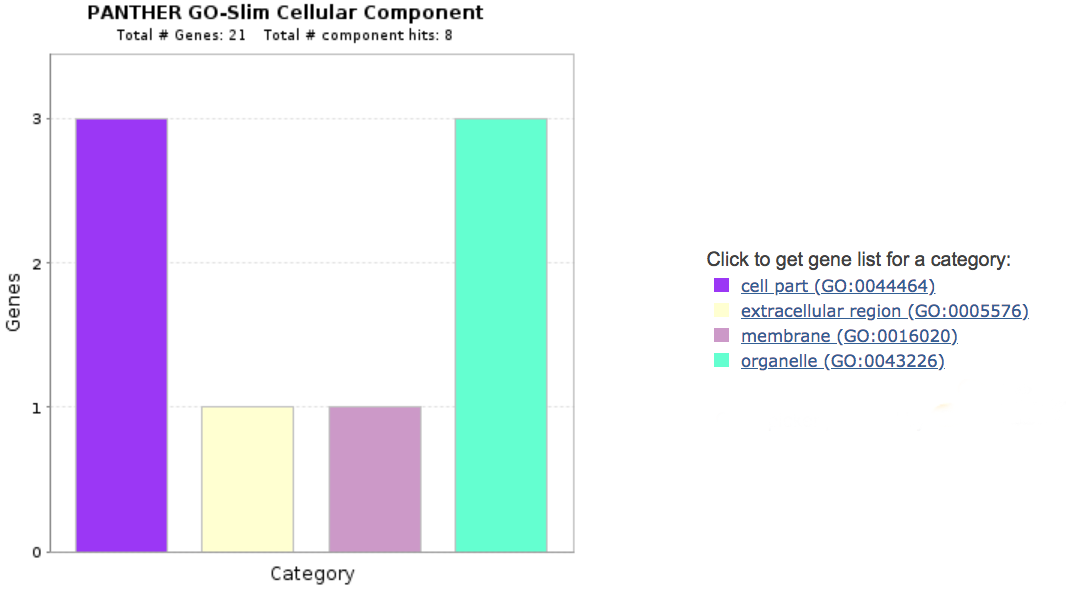
\includegraphics[width=0.9\textwidth]{./Figures/GO/adpd/adpd3}\par
\end{subfigure}
\begin{subfigure}[b]{0.5\linewidth}
\centering
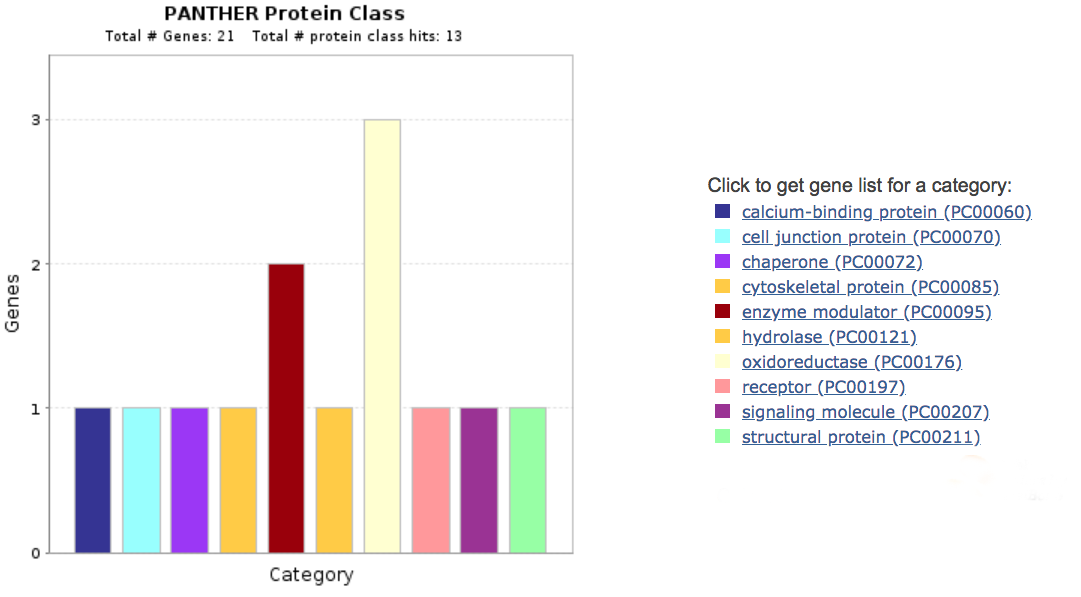
\includegraphics[width=0.9\textwidth]{./Figures/GO/adpd/adpd4}\par
\end{subfigure}%
\begin{caption}
  {Gene ontologies for proteins found in \ref{adpd}.}
\end{caption}
\end{figure}

\subsection{Differentially expressed proteins in comorbid versus non-comorbid Alzheimer's}
\label{sec:comp-diff-expr}

\subsubsection{Common proteins}
\label{subsec:adpdANDad}

{
\small

\begin{itemize}
\item \href{http://www.pantherdb.org/genes/gene.do?acc=HUMAN\%7CHGNC\%3D17056\%7CUniProtKB\%3DQ9Y2J0}{Q9Y2J0}: Rabphilin-3A, function undescribed for humans in PANTHER.
\item \href{http://www.pantherdb.org/genes/gene.do?acc=HUMAN\%7CHGNC\%3D20318\%7CUniProtKB\%3DQ9H4F8}{Q9H4F8}: SPARC-related modular calcium-binding protein 1, associated with the binding of calcium ions.
\item \href{http://www.pantherdb.org/genes/gene.do?acc=HUMAN\%7CHGNC\%3D29393\%7CUniProtKB\%3DQ96Q06}{Q96Q06}: Perilipin-4, function undescribed for humans in PANTHER.
\item \href{http://www.pantherdb.org/genes/gene.do?acc=HUMAN\%7CHGNC\%3D2033\%7CUniProtKB\%3DP78369}{P78369}: Claudin-10,  a tight junction protein known to be found in the plasma membrane.
\item \href{http://www.pantherdb.org/genes/gene.do?acc=HUMAN\%7CHGNC\%3D11280\%7CUniProtKB\%3DQ13501}{Q13501}: Sequestosome-1, known to be associated with protein binding in vacuoles in the cytoplasm.
\item \href{http://www.pantherdb.org/genes/gene.do?acc=HUMAN\%7CHGNC\%3D5246\%7CUniProtKB\%3DP04792}{P04792}: Heat shock protein beta-1, involved in multiple signalling pathways as well as sensory and in particular visual perception.
\item \href{http://www.pantherdb.org/genes/gene.do?acc=HUMAN\%7CHGNC\%3D17972\%7CUniProtKB\%3DQ9NPD7}{A0A087WWT2}: Neuritin, also known as \href{https://www.uniprot.org/uniprot/A0A087WWT2}{NRN1}, function undescribed for humans in PANTHER.
\item \href{http://www.pantherdb.org/genes/gene.do?acc=HUMAN\%7CHGNC\%3D29180\%7CUniProtKB\%3DQ9UPV7}{Q9UPV7}: Unnamed, also known as \href{https://www.uniprot.org/uniprot/Q9UPV7}{PHF24 (PHD Finger Protein 24))}, function undescribed for humans in PANTHER.
\end{itemize}

}

\begin{figure}[H]
\label{adpdANDadfigure}
\begin{subfigure}[b]{0.5\linewidth}
\centering
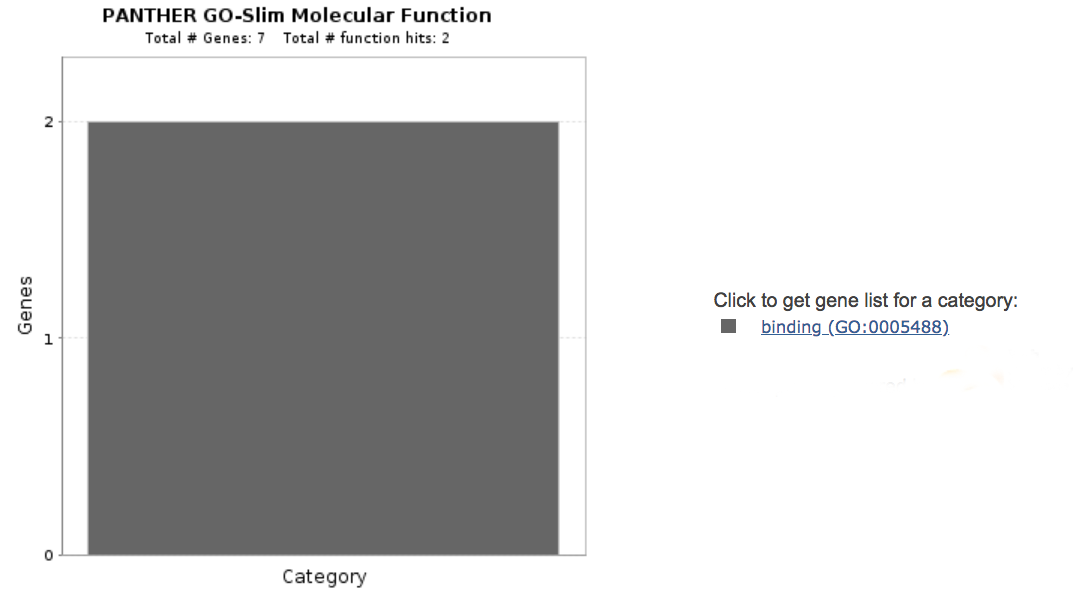
\includegraphics[width=0.9\textwidth]{./Figures/GO/adpdANDad/adpdANDad1}\par
\end{subfigure}
\begin{subfigure}[b]{0.5\linewidth}
\centering
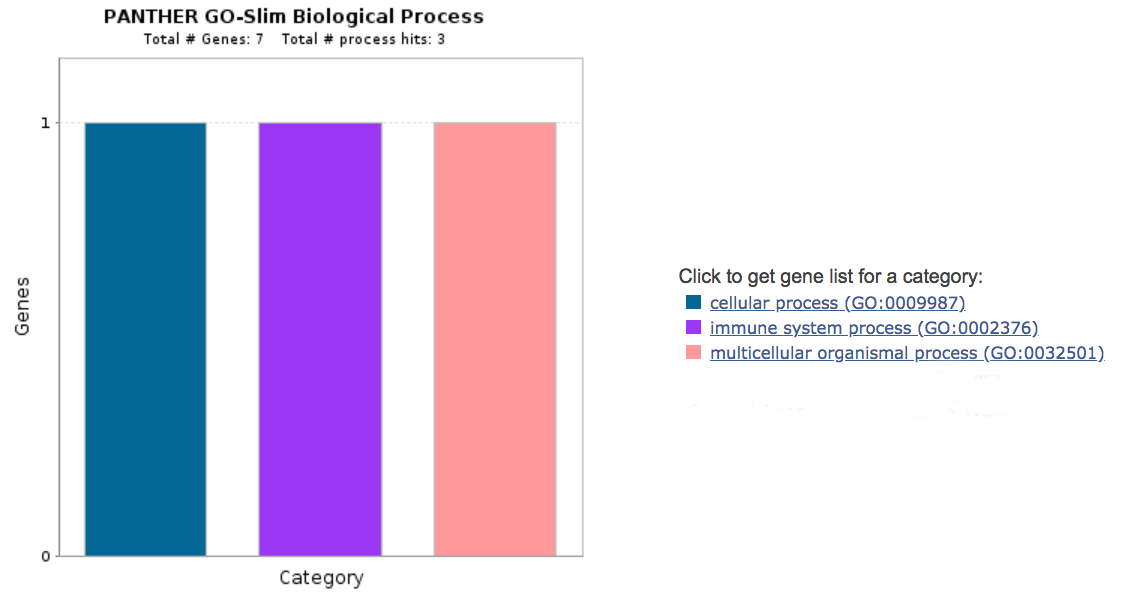
\includegraphics[width=0.9\textwidth]{./Figures/GO/adpdANDad/adpdANDad2}\par
\end{subfigure}\\
\begin{subfigure}[b]{0.5\linewidth}
\centering
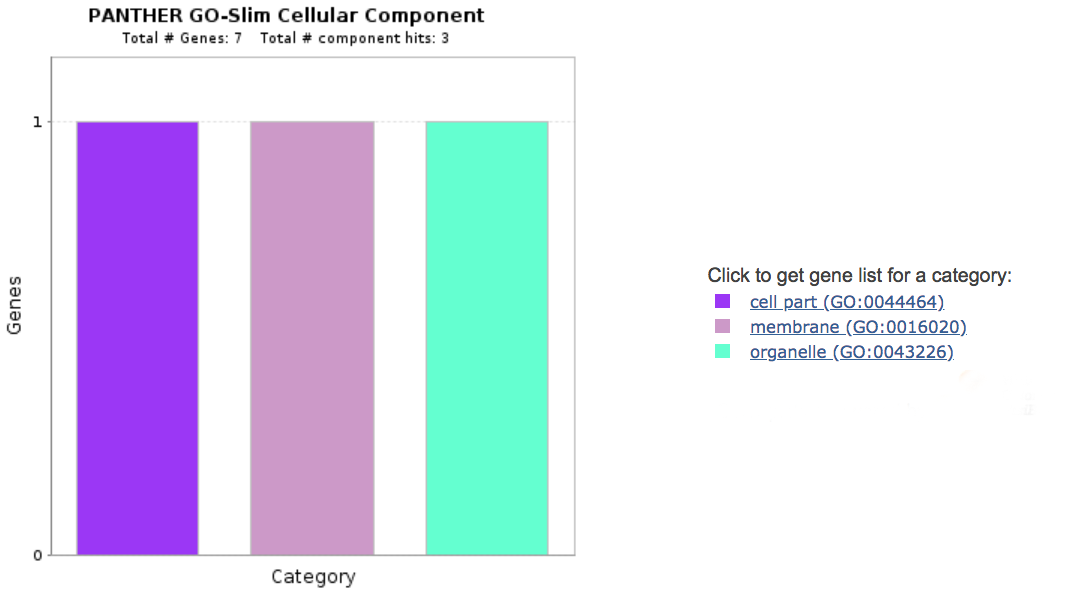
\includegraphics[width=0.9\textwidth]{./Figures/GO/adpdANDad/adpdANDad3}\par
\end{subfigure}
\begin{subfigure}[b]{0.5\linewidth}
\centering
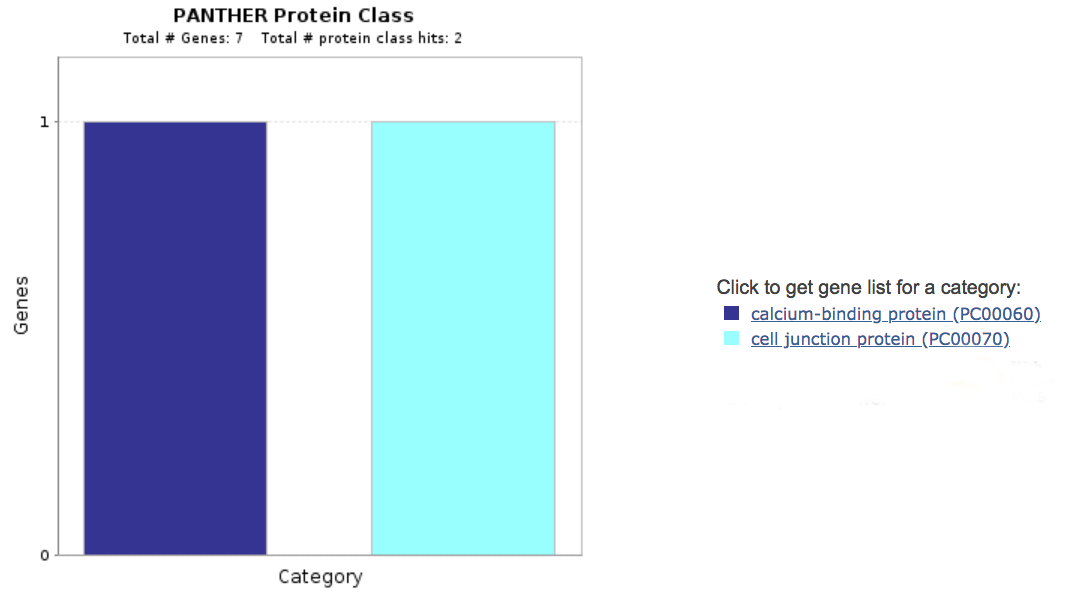
\includegraphics[width=0.9\textwidth]{./Figures/GO/adpdANDad/adpdANDad4}\par
\end{subfigure}%
\begin{caption}
  {Gene ontologies for proteins found in \ref{subsec:adpdANDad}.}
\end{caption}
\end{figure}

\subsubsection{Identified in comorbid but not in non-comorbid}
\label{subsec:adpdNOTad}

{
\small

\begin{itemize}
\item \href{http://www.pantherdb.org/genes/gene.do?acc=HUMAN\%7CHGNC\%3D12684\%7CUniProtKB\%3DO15240}{O15240}: Neurosecretory protein VGF, function undescribed for humans in PANTHER.
\item \href{http://www.pantherdb.org/genes/gene.do?acc=HUMAN\%7CHGNC\%3D9243\%7CUniProtKB\%3DO14829}{O14829}: Serine/threonine-protein phosphatase with EF-hands 1, associated with apoptosis and intracellular signalling.
\item \href{http://www.pantherdb.org/genes/gene.do?acc=HUMAN\%7CHGNC\%3D9476\%7CUniProtKB\%3DQ92743}{Q92743}: Serine protease HTRA1, associated with serine-type proteolysis (peptide and protein breakdown).
\item \href{http://www.pantherdb.org/genes/gene.do?acc=HUMAN\%7CHGNC\%3D13564\%7CUniProtKB\%3DQ92563}{Q92563}: Testican-2, associated with calcium ion binding, and the inhibition of proteolysis.
\item \href{http://www.pantherdb.org/genes/gene.do?acc=HUMAN\%7CHGNC\%3D964\%7CUniProtKB\%3DO75936}{O75936}: Gamma-butyrobetaine dioxygenase, known to be associated with the synthesis of certain vitamins.
\item \href{http://www.pantherdb.org/genes/gene.do?acc=HUMAN\%7CHGNC\%3D17187\%7CUniProtKB\%3DQ99784}{Q99784}: Noelin, a phosphate ion receptor and transporter.
\item \href{http://www.pantherdb.org/genes/gene.do?acc=HUMAN\%7CHGNC\%3D13345\%7CUniProtKB\%3DQ14693}{Q14693}: Phosphatidate phosphatase LPIN1, known to be associated with the regulation of transcription.
\item \href{http://www.pantherdb.org/genes/gene.do?acc=HUMAN\%7CHGNC\%3D3978\%7CUniProtKB\%3DO75891}{O75891}: Cytosolic 10-formyltetrahydrofolate dehydrogenase, a catalyst for the transfer of electrons from one molecule to another (oxidation-reduction reactions).
\item \href{http://www.pantherdb.org/genes/gene.do?acc=HUMAN\%7CHGNC\%3D166\%7CUniProtKB\%3DO43707}{K7EJH8}: Alpha-actinin-4, also known as \href{https://www.uniprot.org/uniprot/K7EJH8}{ACTN4}, associated with the morphogenesis of the extracellular matrix/cytoskeleton.
\item \href{http://www.pantherdb.org/genes/gene.do?acc=HUMAN\%7CHGNC\%3D1470\%7CUniProtKB\%3DQ96RR4}{Q96RR4}: Calcium/calmodulin-dependent protein kinase 2, associated with calcium-mediated synaptic transmission.
\item \href{http://www.pantherdb.org/genes/gene.do?acc=HUMAN\%7CHGNC\%3D1063\%7CUniProtKB\%3DP30043}{P30043}: Flavin reductase (NADPH), another oxidation-reduction catalyst.
\item \href{http://www.pantherdb.org/genes/gene.do?acc=HUMAN\%7CHGNC\%3D8576\%7CUniProtKB\%3DQ15102}{Q15102}: Platelet-activating factor acetylhydrolase IB subunit gamma, specific function undescribed for humans in PANTHER.
\item \href{http://www.pantherdb.org/genes/gene.do?acc=HUMAN\%7CHGNC\%3D20039\%7CUniProtKB\%3DP40123}{P40123}: Adenylyl cyclase-associated protein 2, known to be involved in the organization and regulation of the intracellular actin cytoskeleton in the cytoplasm.
\item \href{http://www.pantherdb.org/genes/gene.do?acc=HUMAN\%7CHGNC\%3D16280\%7CUniProtKB\%3DQ9NQ86}{Q9NQ86}: E3 ubiquitin-protein ligase TRIM36, specific function undescribed for humans in PANTHER.
\item \href{http://www.pantherdb.org/genes/gene.do?acc=HUMAN\%7CHGNC\%3D9064\%7CUniProtKB\%3DQ9UPR0}{Q9UPR0}:  Inactive phospholipase C-like protein 2, associated with GTPase regulation and several intracellular signalling pathways.
\end{itemize}

}

\begin{figure}[H]
\label{adpdNOTadfigure}
\begin{subfigure}[b]{0.5\linewidth}
\centering
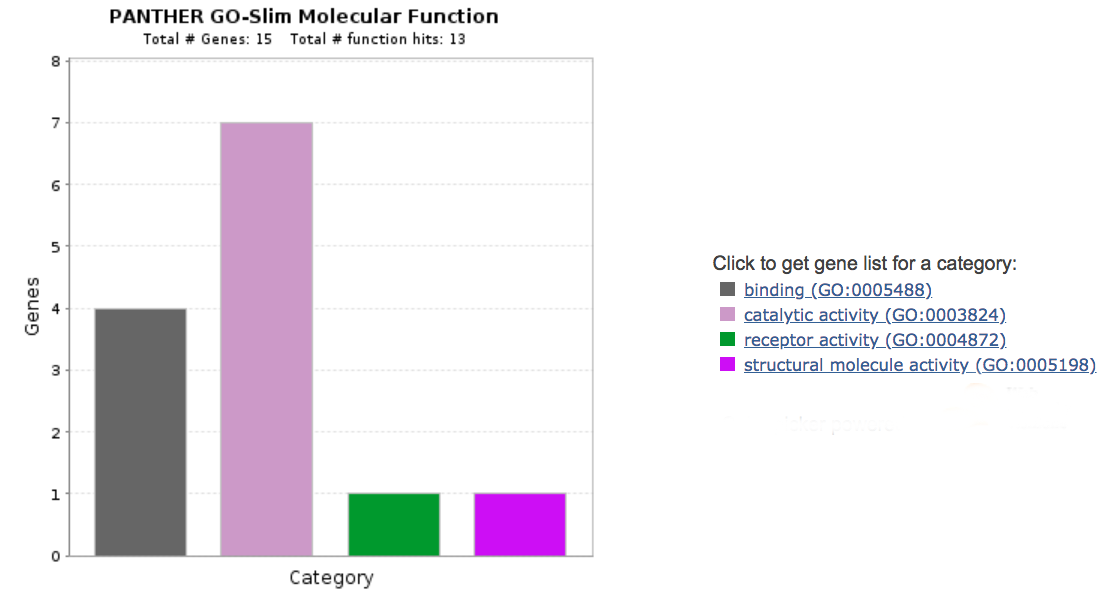
\includegraphics[width=0.9\textwidth]{./Figures/GO/adpdNOTad/adpdNOTad1}\par
\end{subfigure}
\begin{subfigure}[b]{0.5\linewidth}
\centering
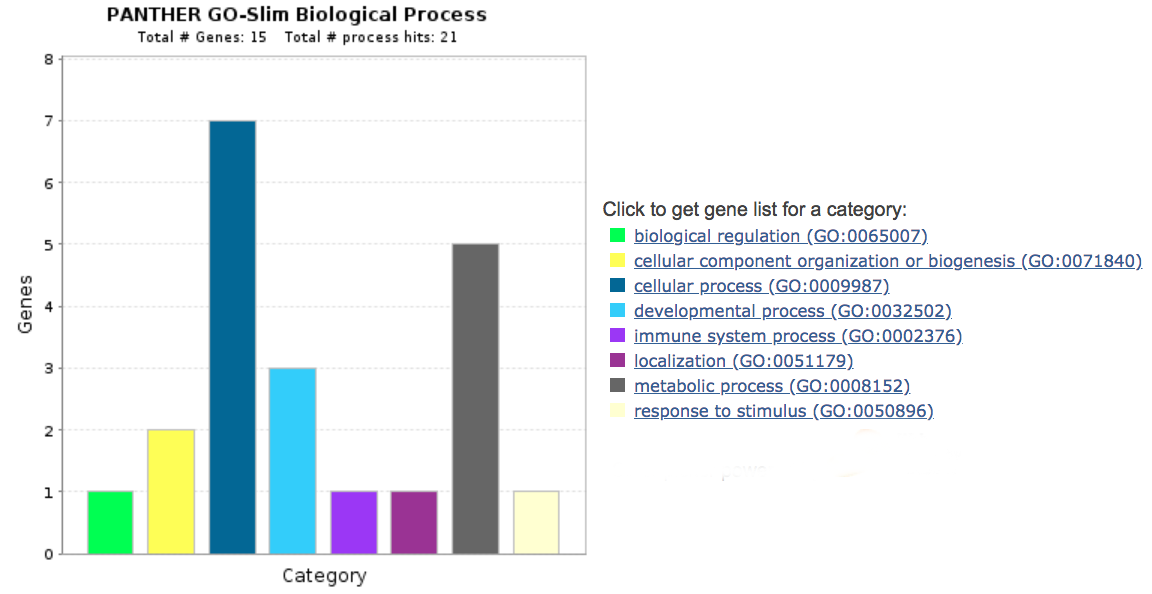
\includegraphics[width=0.9\textwidth]{./Figures/GO/adpdNOTad/adpdNOTad2}\par
\end{subfigure}\\
\begin{subfigure}[b]{0.5\linewidth}
\centering
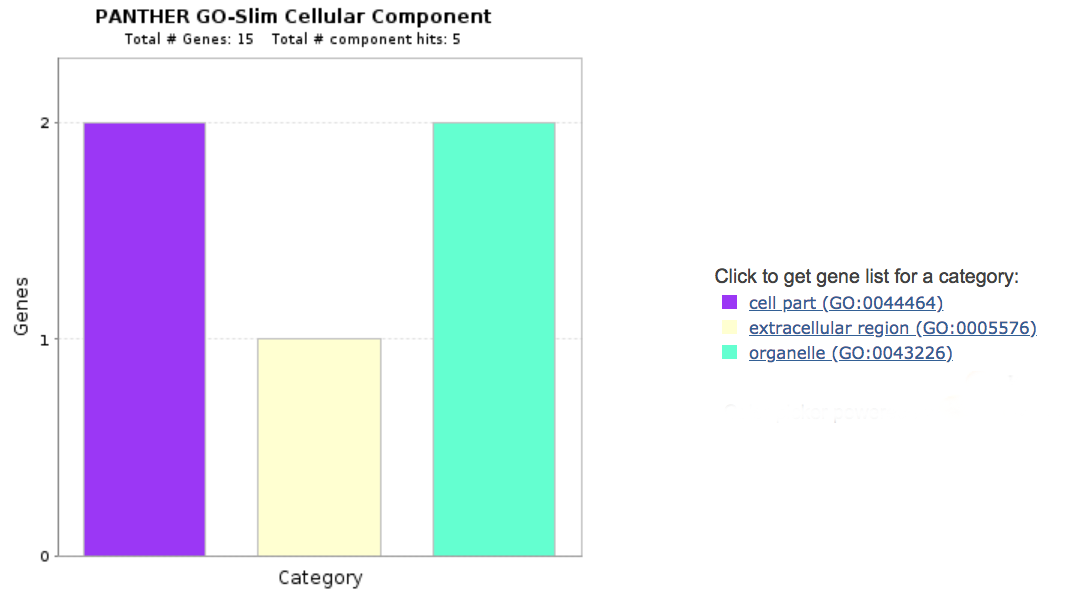
\includegraphics[width=0.9\textwidth]{./Figures/GO/adpdNOTad/adpdNOTad3}\par
\end{subfigure}
\begin{subfigure}[b]{0.5\linewidth}
\centering
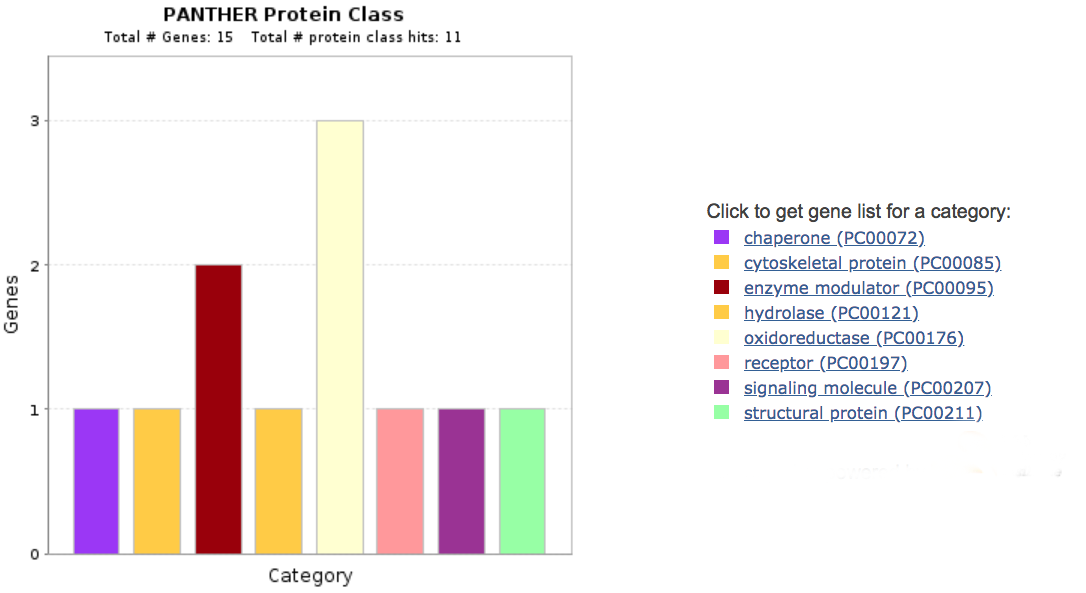
\includegraphics[width=0.9\textwidth]{./Figures/GO/adpdNOTad/adpdNOTad4}\par
\end{subfigure}%
\begin{caption}
  {Gene ontologies for proteins found in \ref{subsec:adpdNOTad}.}
\end{caption}
\end{figure}


\subsubsection{Identified in in non-comorbid but not in comorbid}
\label{subsec:adNOTadpd}

{\small

\begin{itemize}
\item \href{http://www.pantherdb.org/genes/gene.do?acc=HUMAN\%7CHGNC\%3D6893\%7CUniProtKB\%3DP10636}{P10636}: Microtubule-associated protein tau, associated with microtubule binding and neuron projection.
\item \href{http://www.pantherdb.org/genes/gene.do?acc=HUMAN\%7CHGNC\%3D2318\%7CUniProtKB\%3DQ9HCH3}{Q9HCH3}: Copine-5, function undescribed for humans in PANTHER.
\item \href{http://www.pantherdb.org/genes/gene.do?acc=HUMAN\%7CHGNC\%3D4638\%7CUniProtKB\%3DP09211}{P09211}: Glutathione S-transferase P, function undescribed for humans in PANTHER.
\item \href{http://www.pantherdb.org/genes/gene.do?acc=HUMAN\%7CHGNC\%3D9099\%7CUniProtKB\%3DQ9UIW2}{Q9UIW2}: Also known as \href{https://www.uniprot.org/uniprot/Q9UIW2}{PLXNA1 (Plexin-A1)}, associated with axon guidance mediated by semaphorins, nervous system development, signal transducer activity, receptor activity, GTPase activity, pyrophosphatase activity, and many others.
\item \href{http://www.pantherdb.org/genes/gene.do?acc=HUMAN\%7CHGNC\%3D11444\%7CUniProtKB\%3DP61764}{P61764}: Syntaxin-binding protein 1, also known as \href{https://www.uniprot.org/uniprot/P61764}{STXBP1}, associated with synaptic vesicle exocytosis and trafficking (as part of synaptic transmission).
\item \href{http://www.pantherdb.org/genes/gene.do?acc=HUMAN\%7CHGNC\%3D2451\%7CUniProtKB\%3DP48729}{P48729}: Also known as \href{https://www.uniprot.org/uniprot/P48729}{CSNK1A1 (Casein kinase I isoform alpha))}, associated with protein kinase activity. Well known to be associated with Parkinson's disease.
\item \href{http://www.pantherdb.org/genes/gene.do?acc=HUMAN\%7CHGNC\%3D16753\%7CUniProtKB\%3DP30041}{P30041}: Peroxiredoxin-6, an enzyme which catalyzes the oxidation via hydrogen peroxide.
\item \href{http://www.pantherdb.org/genes/gene.do?acc=HUMAN\%7CHGNC\%3D8923\%7CUniProtKB\%3DO43175}{O43175}: D-3-phosphoglycerate dehydrogenase, associated with the synthesis of serine and glycine.
\item \href{http://www.pantherdb.org/genes/gene.do?acc=HUMAN\%7CHGNC\%3D19129\%7CUniProtKB\%3DQ9Y617}{Q9Y617}: Phosphoserine aminotransferase, also associated with the synthesis of serine and glycine, as well as pyridoxal-5 phosphate synthesis and vitamin B6 metabolism.
\item \href{http://www.pantherdb.org/genes/gene.do?acc=HUMAN\%7CHGNC\%3D2482\%7CUniProtKB\%3DP04080}{P04080}: Cystatin-B, known to be a cysteine protease inhibitor.
\item \href{http://www.pantherdb.org/genes/gene.do?acc=HUMAN\%7CHGNC\%3D4288\%7CUniProtKB\%3DO95452}{O95452}: Gap junction beta-6 protein, associated with gap junction channel activity in the plasma membrane.
\item \href{http://www.pantherdb.org/genes/gene.do?acc=HUMAN\%7CHGNC\%3D10661\%7CUniProtKB\%3DP31431}{P31431}: Syndecan-4, a cytoskeletal protein involved in cell adhesion and the extracellular matrix, as well as membrane-bound signalling.
\item \href{http://www.pantherdb.org/genes/gene.do?acc=HUMAN\%7CHGNC\%3D18304\%7CUniProtKB\%3DQ14019}{Q14019}: Coactosin-like protein, involved in the intracellular actin cytoskeleton, in particular with the binding of actin as well as a cytoskeletal component itself.
\item \href{http://www.pantherdb.org/genes/gene.do?acc=HUMAN\%7CHGNC\%3D19663\%7CUniProtKB\%3DQ9UBI6}{Q9UBI6}: Guanine nucleotide-binding protein G(I)/G(S)/G(O) subunit gamma-12, involved in GTPase activity, protein binding, and numerous signalling pathways.
\item \href{http://www.pantherdb.org/genes/gene.do?acc=HUMAN\%7CHGNC\%3D20983\%7CUniProtKB\%3DQ8N987}{Q8N987}: N-terminal EF-hand calcium-binding protein 1, known to be found in the cytoplasm and involved in the regulation of cellular metabolism, given the naming presumably via the binding of calcium. Otherwise little else appears to be described in PANTHER.
\item \href{http://www.pantherdb.org/genes/gene.do?acc=HUMAN\%7CHGNC\%3D29167\%7CUniProtKB\%3DQ9Y2K5}{B5MCG9}: R3H domain-containing protein 2, also known as \href{https://www.uniprot.org/uniprot/B5MCG9}{R3HDM2}, function unknown in humans.
\end{itemize}

}

\begin{figure}[H]
\label{adNOTadpdfigure}
\begin{subfigure}[b]{0.5\linewidth}
\centering
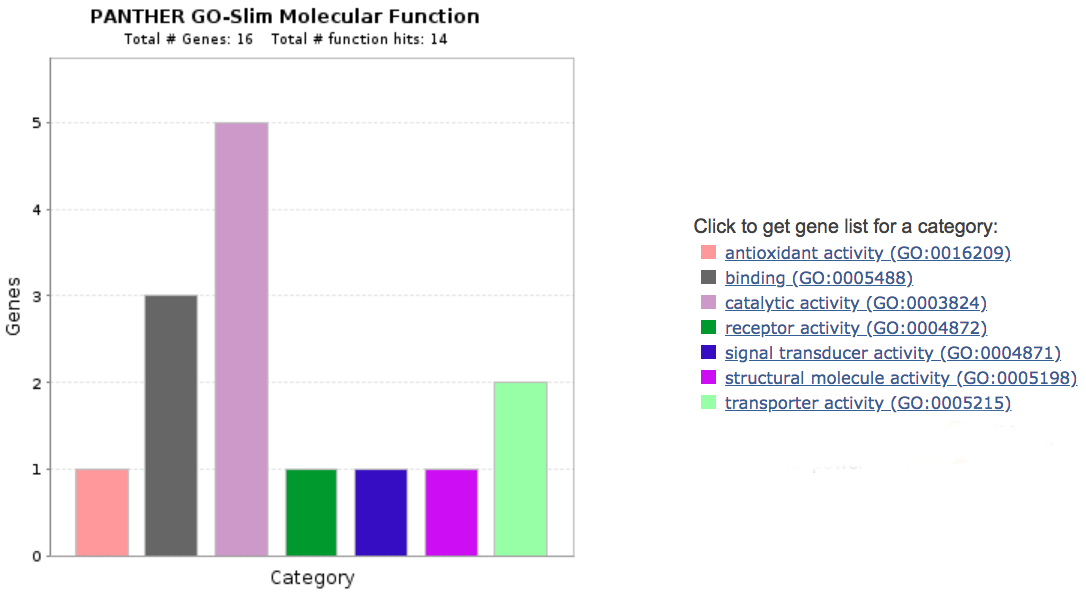
\includegraphics[width=0.9\textwidth]{./Figures/GO/adNOTadpd/adNOTadpd1}\par
\end{subfigure}
\begin{subfigure}[b]{0.5\linewidth}
\centering
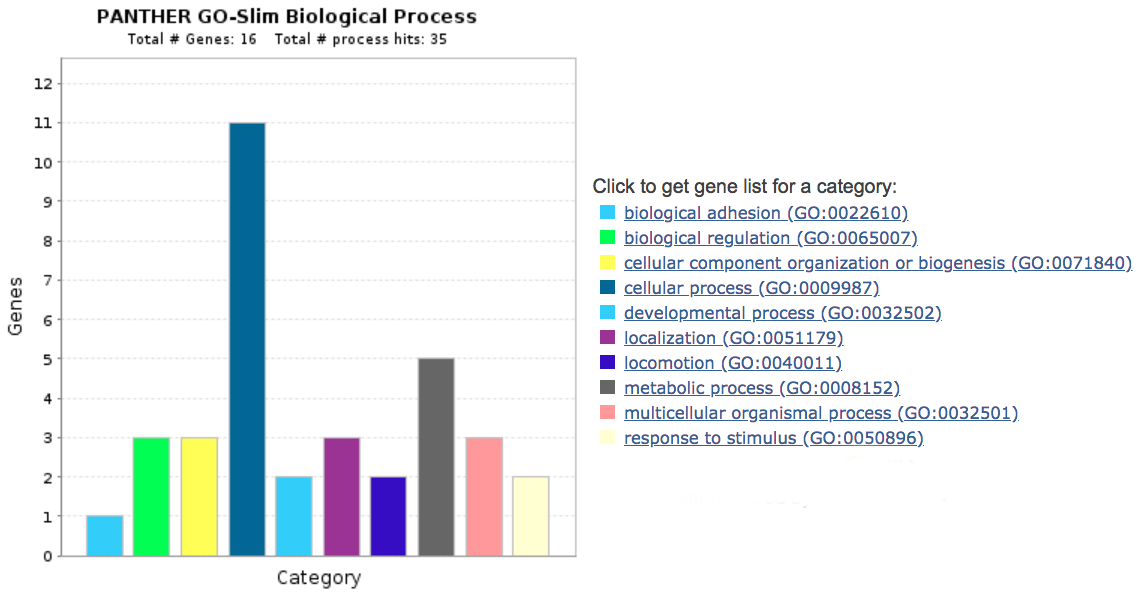
\includegraphics[width=0.9\textwidth]{./Figures/GO/adNOTadpd/adNOTadpd2}\par
\end{subfigure}\\
\begin{subfigure}[b]{0.5\linewidth}
\centering
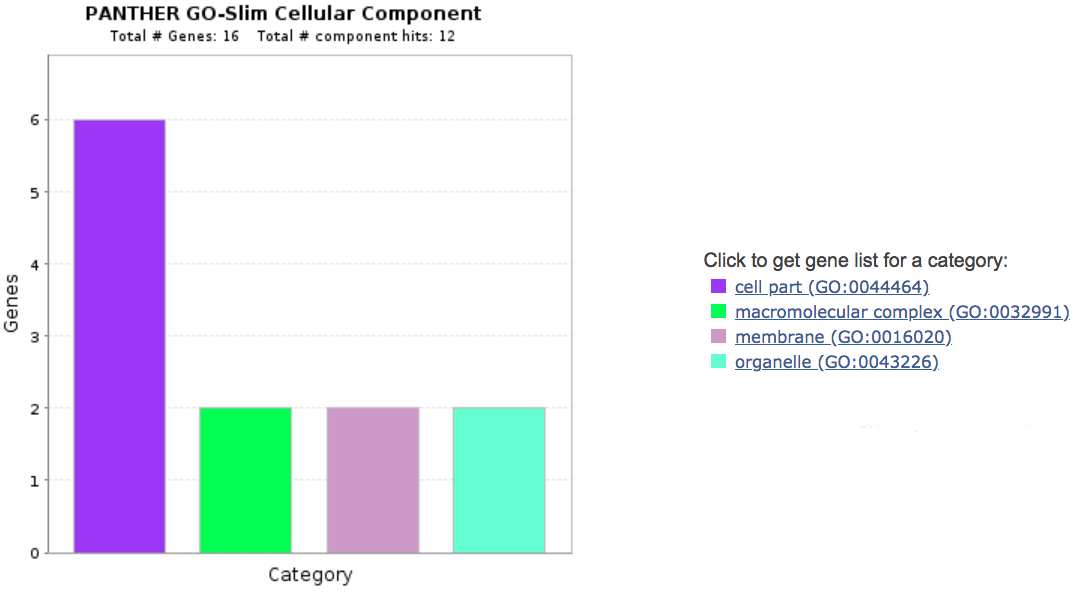
\includegraphics[width=0.9\textwidth]{./Figures/GO/adNOTadpd/adNOTadpd3}\par
\end{subfigure}
\begin{subfigure}[b]{0.5\linewidth}
\centering
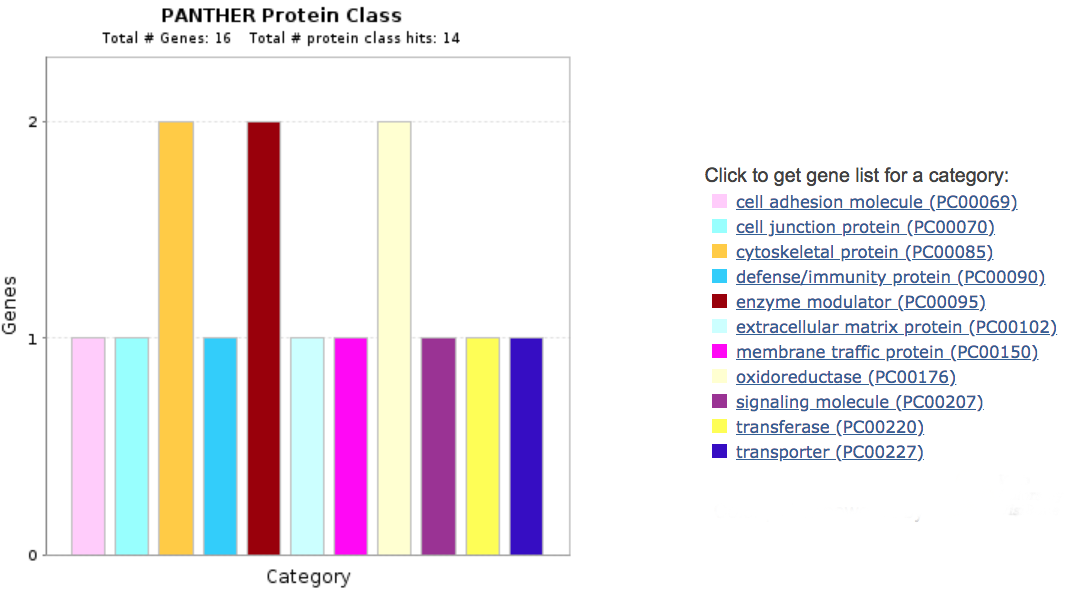
\includegraphics[width=0.9\textwidth]{./Figures/GO/adNOTadpd/adNOTadpd4}\par
\end{subfigure}%
\begin{caption}
  {Gene ontologies for proteins found in \ref{subsec:adNOTadpd}.}
\end{caption}
\end{figure}

\textbf{Comments:} First, it is very surprising that the tau protein associated so closely with Alzheimer's is not Identified as differentially expressed among the comorbid group. It is also strange (but less so, since we don't expect manifestation of Parkinson's in the frontal cortex) that the casein kinase associated with Parkinson's is not identified as differentially expressed among the comorbid group.\\

What is perhaps strangest here is the relatively small overlap between genes identified as differentially expressed in both the comorbid and non-comorbid group, and that there are so many genes identified as differentially expressed in the non-comorbid but not in the comorbid group. This is because we expect the comorbid group to be manifesting the same disease as the non-comorbid group, plus another disease, such that the differentially expressed genes in the comorbid group would be expected to be approximately a strict superset of those in the non-comorbid group -- yet this is not what happened at all.\\

This counter-intuitive finding invites deeper scrutiny of our methodology as well as the assumptions implicit in using that methodology. However, if the finding was valid, it seemingly would possibly be of genuine interest to domain experts.\\

\subsection{Summary}
\label{sec:summary}

Some of our findings, e.g. that tau protein is differentially expressed, and that Parkinson's does not seem to manifest in the frontal cortex, correspond well to existing research. Others are more surprising, some even counterintuitive. There are other aspects of our results which argue in our favor. For example, we found several proteins involved in serine synthesis and metabolism to be differentially expressed, which corresponds to previous research linking Alzheimer's and serine\cite{HASHIMOTO2004385, KATSOURI2011S702, Madeira2015, clinicaltrials.gov}. The same is also true of the identification of GTPase proteins as possibly relevant\cite{Nishimoto1993, Bolognin2014, Aguilar2017}.\\

Based on our findings, we would also recommend future studies of Rabphilin-3A and Perilipin-4 and their relationships to Alzheimer's and Parkinson's to follow those which have already been made \cite{TAN201429, Stanic2015, STANIC201754} \cite{10.3389/fnins.2018.00397, Shimabukuro2016, Heck2014} (as well as updates of the PANTHER database to more fully reflect current knowledge of these proteins). In any case, the existence of prior work studying these connections suggests at the very least that our analysis is not completely unreasonable in finding these proteins to possibly be important.

\pagebreak

\bibliographystyle{siam}
\bibliography{bibliography}
\addcontentsline{toc}{section}{References}

\end{document}

